\section{Konzeptentwicklung für die Labordigitalisierung}
\label{sec:konzeptentwicklung}

In diesem Abschnitt werden die Konzepte erläutert, die im Verlauf des Projekts erarbeitet werden. Es werden zwei Konzepte entwickelt, die auf das gesamte verfahrenstechnische Labor angewendet werden können. Die Konzepte schließen sich nicht gegenseitig aus, sondern bauen aufeinander auf. Als erstes wird das Konzept erläutert, welches auf die Verwendung einer Datenbank verzichtet. 
Als zweites wird ein Konzept erläutert, in dessen Zentrum sich eine Datenbank befindet. Die Datenübertragungswege sind durchnummeriert. Des Weiteren gibt es pro vorgestelltem Entwurf alternative Datenübertragungswege oder Lösungen die jedoch nicht betrachtet werden. \\

Es wurden \textbf{Anforderungen} für die Konzeptionierung definiert, die nachfolgend aufgelistet sind: 


\begin{enumerate}[leftmargin = 1.2em, label = \textbullet , itemsep = 0.1em]
\item Das Konzept soll für das verfahrenstechnische Labor allgemeingültig sein.
\item Die \glqq digitalen Kompetenzen\grqq{} der Studierenden sollen maximiert werden, ohne die fachlichen Kompetenzen signifikant zu reduzieren, durch 
\item ein Minimum an Automatisierung.

	\begin{enumerate}[leftmargin = 1.2em, label = -- , itemsep = 0.1em]
	\item Unter Automatisierung kann z.B.  die Manipulation von Daten, wie die Detektion von Ausreißer und dessen Entfernung, genaue Leitfäden in der Handhabung, die keine Fehler mehr zulassen o.ä., verstanden werden.
\end{enumerate}
	
\item Der monetäre Aufwand soll minimal sein.
\item Möglichkeiten der Datenerfassung/Signalverarbeitung sollen eruiert werden. 
\item Die inkrementelle Implementation von Applikationen im Rahmen von Industrie 4.0 und Big Data (KI, Digital Twin etc.) soll tendenziell möglich sein.
\item Cloud Computing soll in Betracht gezogen werden.

	\begin{enumerate}[leftmargin = 1.2em, label = -- , itemsep = 0.1em]
	\item Erster Schritt der Umsetzung: Speicherung der Rohdaten auf der HAW Cloud
	\item Zweiter Schritt der Umsetzung: Cloudnutzung, gemäß des Impulsvortrags zum Digitalisierungsfond $\Rightarrow$ Amazon, Google, Microsoft Azure
	\end{enumerate}
	
\item Die gesamte Protokollierung der Studierenden soll in Zukunft digital sein.
\end{enumerate}


\subsection{Konzeptentwurf 3.0 (ohne Datenbank)}

In der Abbildung \ref{digitalisierungskonzept_ohne_db} ist ein Digitalisierungsentwurf ohne die Verwendung einer Datenbank dargestellt. Die Feldebene auf der linken Seite der Abbildung und die Softwareebene sind durch eine \textcolor{orange}{Strich-Doppelpunkt Linie} voneinander getrennt. Der Feldebene sind Feldgerätedaten und Daten, die manuell eingegeben werden müssen, zugeordnet. Die Datenerfassung und das Schreiben von Messwertdaten in CSV-Dateien, die Auswertung und die Protokollierung sind der Softwareebene zugeordnet. CSV-Dateien sind Textdateien, die in ein Tabellenkalkulationsprogramm importiert werden können, deren Spalten durch ein frei wählbares Trennzeichen getrennt sind. In den folgenden sechs Absätzen werden die Elemente der Feld- und Softwareebene erläutert.\\

\bild{1.0}
{digitalisierungskonzept_ohne_db.png}
{0em}
{Digitalisierungsentwurf ohne Datenbank}
{Digitalisierungsentwurf ohne Datenbank}
{digitalisierungskonzept_ohne_db}

\paragraph*{Feldgerätedaten} Die Feldgerätedaten, wie z.B. welche Anlage, Maschine, Messeinrichtung und deren Messwertdaten sind der Feldebene zugeordnet. Auch die Signale oder Daten, die von einem Gerät erfasst werden, sind der Feldgeräteebene zugeordnet.

\paragraph*{Manueller Dateninput} Dem manuellen Dateninput sind alle Daten zugeordnet, die  dokumentiert werden müssen. Unter den zu dokumentierenden Daten können Versuchsparameter wie die Partikeldichte, die Schüttgutmasse etc. sein. Organisatorische Daten sind ebenfalls zu dokumentieren und können bspw. die Gruppen ID, Anwesenheitsinfomationen o.ä. sein.

\paragraph*{Datenerfassung} Für die Datenerfassung, auch Datenakquisition (DAQ~, \textit{engl. data acquisition}) bieten sich Lösungen mit einer grafischen Benutzeroberfläche (\textit{engl. graphic user interface, GUI}) an. Die Datenerfassung kann mittels einer grafischen Programmiersprache wie z.B. LabVIEW realisiert werden oder mit einer textbasierten Programmiersprache wie bspw. Python \cite{low-cost_daq}. Des Weiteren ist eine Datenerfassungssoftware der Gerätehersteller ebenfalls denkbar, (z.B. Laserbeugung-Partikelgrößenanalyse). Datenmanipulationen während der Datenerfassungen müssen dokumentiert und nachvollzogen werden können.

\paragraph*{Messwert-Datalogging} Die diskreten oder kontinuierlichen Daten von Messeinrichtungen können in eine Datei geschrieben werden. Prinzipiell sind zwei Datenformate möglich, das schreiben der Daten im ASCII-Format oder binär. Das entscheidende Auswahlkriterium ist der Speicherbedarf (vgl. Abbildung \ref{fig:speicherbedarf_vergleich} im Anhang  \cite[S. 44]{speicherbedarf_vergleich_binär-ascii}). Eine etablierte Dateiform für Messungsdaten ist die Speicherung in Text-Dateien, genannt CSV-Datei. CSV steht für comma separated value. Die Spalteneinträge sind durch ein Spaltentrennzeichen (engl. \textit{delimiter}) getrennt. Als Spaltentrennzeichen kann neben dem Komma ein beliebiges Zeichen gewählt werden. Die Lösung des Dataloggings in CSV-Dateien hat einen geringen Speicherbedarf (z.B. im vgl. zu Excels *.xlsx-Dateien), da nur \glqq Nutzdaten\grqq{} sowie delimiter, jedoch keine Formatierungsinformation oder der Gleichen vorhanden sind \cite[S. 319]{HandbuchfuerLabview}.

\paragraph*{Auswertung} Die Auswertung kann je nach Vorgabe mit entsprechenden Softwarelösungen (Excel, Matlab, Python etc.) realisiert werden. Die Rohdaten (\textit{engl. raw data}) aus den CSV-Dateien können bspw. in Excel importiert und weiter verarbeitet werden.

\paragraph*{Protokollierung} Das Digitalisierungskonzept welches ohne die Nutzung einer Datenbank auskommt, nutzt zur Datenarchivierung und Protokollierung ein sog. Elektronisches Labor Notebook (ELN), auch Labor Journal genannt. In ELN's können Eingabemasken für diskrete Daten (Versuchsparameter, organisatorische Informationen...) generiert werden. Des Weiteren lassen sich gängige Dateiformate per drag and drop zur Dokumentation in ein ELN importieren \cite[S.44 f.]{ELN_laborjournal}.\\

Die durch die Sensoren erfassten Messwerte werden, z.B. über eine RS-232 Schnittstelle, an die Datenerfassungssoftware übertragen (1). Als Datenerfassungssoftware könnte beispielsweise LabVIEW genutzt werden. Die Versuchssinformationen, Zeitreihendaten und Beobachtung während der Versuche können in der Datenerfassungssoftware aufgenommen werden (2). Die erfassten Daten und ggf. Beobachtungen, werden in eine Textdatei (CSV) geschrieben (3). Im englischen Sprachgebrauch wird ein Punkt als Dezimaltrennzeichen verwendet, woraus die Verwendung des Kommas als delimiter keinem Konflikt gegenübersteht. Im deutschsprachigem Raum ist das Komma jedoch nicht als delimiter zum empfehlen \cite[Vorwort]{HandbuchfuerLabview}. Als delimiter für die Spalten in der Textdatei bietet sich das \texttt{Tabualtor} Zeichen an. Es ist gefordert, dass die generierten CSV-Dateien schreibgeschützt sein sollen. Eine Speicherung der Rohdaten soll auf die HAW Cloud erfolgen. Die Rohdaten der Versuche können für die Auswertung bspw. in Excel importiert (4) und sollen dem Protokoll als Anlage angehängt werden (5). Alle zweckmäßigen Datenmanipulationen, die auf den Pfaden 3 bis 6 durchgeführt werden, müssen bekannt und nachvollziehbar dokumentiert werden. Zweckmäßige Datenmanipulationen könnten Glättungsoperationen der Daten, wie der gleitender Mittelwert, die Entfernung von Ausreißern, das Logarithmieren etc. sein.

\subsection{Konzeptentwurf 4.0 (mit Datenbank und Softwarevernetzungsmöglichkeiten)}

In der Abbildung \ref{digitalisierungskonzept_mit_db} ist eine Erweiterung des zuvor dargestellten Konzepts dargestellt. Im Zentrum dieses Entwurfs steht die Verwendung einer \textcolor{OliveGreen}{Datenbank}. Der Softwareebene wurden bei diesem Konzept drei Elemente hinzugefügt. Nachfolgend werden die drei Elemente erläutert.

\bild{1}
{digitalisierungskonzept_mit_db.png}
{0em}
{Digitalisierungsentwurf mit Datenbank}
{Digitalisierungsentwurf mit Datenbank}
{digitalisierungskonzept_mit_db}



\paragraph*{Datenbank} Es könnte eine lokale oder eine cloudbasierte Datenbank zum Einsatz kommen. Auf dem Mark gibt es Dienstleister, die cloudbasierte Lösungen anbieten. Deren Geschäftsmodelle werden X-as-a-Service gennant. Das X dient als Platzhalter für Plattform, Database, Infrastructure, Software etc. \cite{cloudcomputing_insider}. Die Vorteile und Nachteile von Plattform- oder Database-as-a-Service sind in der Tabelle \ref{xaas} aufgelistet \cite{cloudcomputing, dbmserklaert, cloudcomputing_insider}, werden im Rahmen dieser Arbeit jedoch nicht näher erläutert. 

\begin{table}[t]
\caption{Vor- und Nachteile der Nutzung von Database- oder Plattform-as-a-Service, gemäß der Quellen \cite{cloudcomputing, dbmserklaert, cloudcomputing_insider}} \label{xaas}
\begin{center}
\begin{tabularx}{1\textwidth}{X|X}
Vorteile & Nachteile \\ \toprule
+ \,Kostenersparnis & - \,Abhängigkeit vom Dienstleister\\
\quad \textbullet \,Desaster Recovery Maßnahmen & \quad \textbullet \,Unzureichende Kapazitäten \\
\quad \textbullet \,Updates, Wartung, Instandhaltung & \quad \textbullet \,Insolvenz \\
\quad \textbullet \,Infrastruktur 									& \quad \textbullet \,Kundenservice \\
\quad \textbullet \,Software 										&  - \,Datenschutz \\
\quad \textbullet \,Personalkosten 	& \quad \textbullet \,Servicestandort oft nicht in EU/Dt.  \\
+ \,Infrastuktur 												& - \,Datensicherheit (Datenverlust) \\
\quad \textbullet \,Rechenleistung								& - \,eigene IT-Kompetenz \\
\quad \textbullet \,Speichekapazität							& - \,Infrastuktur \\
\quad \textbullet \,Netzwerkkapazität 						& \quad \textbullet \,Latenzzeiten \\
+ \,Anpassbar- und Skalierbarkeit 				& \quad \textbullet  \,lokale Ausfälle \\
+ \,Gut kalkulierbare Fixkosten 					& \quad \textbullet  \,lokale Strom- oder Netzwerk Ausfälle\\
+ \,Sicherheit in Bezug.. 								& \\
\quad \textbullet \,auf Mitarbeiter 								& \\
\quad \textbullet \,Dezentralität  & \\
\quad \enspace $\cdot$  Schutz vor lokale Hackerangriffe & \\
\quad \enspace $\cdot$  social hacking Prävention & \\
+ \, Portfoliosoftware Kompatibilität & \\
\end{tabularx}
\end{center}
\end{table}

\paragraph*{Digital Twin} Es existieren verschiedene Formen des sog. \glqq digitalen Zwillings\grqq{} (\textit{engl. Digital Twins}). Mittels \textit{Digital Twins} können Produkte, Produktionsabläufe oder ein gesamter Prozess, durch die Kopplung von Produktions- und Produkt Twin, abgebildet und somit optimiert werden. Mittels Digital Twins lassen sich sogenannte Soft-Sensoren integrieren (angewandte numerische Simulation). In Produktionsprozessabschnitten, in denen die Bedingungen es nicht erlauben einen realen Langzeitsensor zu implementieren, können, mittels Digital Twins, Sensoren in Simulationssoftware generiert werden, die mit einem Prozess synchronisiert sind, um Totzeiten zu verringern oder zu eliminieren, bis schlechte Produktionsbedingungen detektiert werden können. Dadurch kann die Effizienz eines Prozesses signifikant gesteigert werden kann. Für die Simulation mittels Digital Twins werden Prozess-, Rohstoff- und geometrische Daten benötigt. Die Form der Randbedingungen können vielfältig sein und unterscheiden sich je nach Simulationsobjekt. Randbedingungen könnten Parameter der Umgebung betreffend, materialabhängige Parameter oder Parameter, die der Wertschöpfungskette zugehörig sind, sein. Als Beispiel für Parameter der Wertschöpfungskette kann ein tendenziell auftretender Rohstoffengpass durch Lieferverzug seitens des Zulieferers genannt werden \cite{digitwin_prozessmodellierung}. Weitere Informationen ist weiterführenden Fachliteratur zu entnehmen. \\


\paragraph*{Künstliche Intelligenz} Ein Teilgebiet der Informatik ist das Themengebiet der \glqq künstlichen Intelligenz\grqq{} (KI, \textit{engl. artificial intelligence, AI}). Teilgebiete der Künstlichen Intelligenz sind das \textit{Machine Learning} (ergänzung im Anhang), \textit{Robotik}, sog. \textit{Expertensysteme}, Mustererkennung, die Verarbeitung natürlicher Sprache oder maschinelles Übersetzen (deepl.com) \cite{infos_teilgebiete_ai}. 

Die potenziellen Fähigkeiten von KI Applikationen sind das Lernen, Planen und Problemlösen. Die Ansätze sind jedoch humanzetriert, zur Unterstützung der Menschen, bei ihren Tätigkeiten. Präzisiert bedeutet das \cite[S. 5]{techszenario_i40}:

\begin{center}
\begin{tabularx}{1\textwidth}{p{0,45\textwidth}|X}
\hspace{0,5em} \textbullet \,Wissenserwerb & \hspace{0,5em} \textbullet \,kognitives Erfassen und Automatisieren\\
& \hspace{1em} logischer Schlussfolgerungen\\[4pt]
\hspace{0,5em} \textbullet \,Maschinenlernen & \hspace{0,5em} \textbullet \,Planung und Ausführung industrieller \\
& \hspace{1em} Automatisierungsprozesse \\[4pt]
\hspace{0,5em} \textbullet \,Bild- und Spracherkennung &\hspace{0,5em} \textbullet \,Mustererkennung \\
\end{tabularx}
\end{center}




%Einige Algorithmen müssen angelernt werden (\textit{engl. \textbf{supervised} or \textbf{semi-supervised}}), z.B. das vom Google-Brain-Team entwickelte open-source Modell, Tensor Flow \cite{tensorflow_framework}. Andere werden nicht angelernt und generieren Ihren Algorithmus autonom (\textit{engl. \textbf{unsupervised}}; vgl. \ref{fig:supervised_machinelearning} im Anhang). \textbf{Supervised Learning}  (vgl. Abbildung \ref{fig:supervised_machinelearning} im Anhang) bedeutet, dass Datensätze vorgegeben werden und zugleich deren Lösung bzw. Klassifizierungen. Anhand des dadurch generierten Algorithmus werden unbekannte Datensätze klassifiziert. Je nach verwendetem Algorithmus können Klassifizierungen binär wie Spam, nicht Spam; Mann, Frau oder Multi-Class-Klassifizierungen, wie z.B. Porsche, Mercedes, VW, .... sein. \textbf{Semi-Supervised Learning} Algorithmen verändern ihren angelernt Algorithmen, bzw. können Ihren Algorithmus, anhand der unvalidierten Daten, die sie nach dem anlernen erhalten, optimieren. KI Algorithmen benötigen große, Datenmengen. Einfache KI's benötigen zusätzlich strukturierte Daten, damit ist die Verfügbarkeit der Daten in Datenbanken gemeint. Die neusten, komplexen \cite{unstrukturierte_daten_ki} maschine learning Algorithmen können auch mit unstrukturierten Daten verwertbare Ergebnisse generieren, doch es gilt stets GIGO, \glqq garbage in, garbage out!\grqq{} Die Güte der Ergebnisse einer KI wird durch die Güte der Ausgangsdaten bestimmt, demnach ist die Wahrscheinlichkeit mit strukturierten Daten ein sinnvolles, aussagekräftiges Ergebnis zu erzielen wahrscheinlich höher.
%Es existiert noch eine vierte Kategorie, die \textbf{Reinforced Learning} Algorithmen. Diese Algorithmen unterscheiden sich von den unsupervised Algorithmen in der Art, dass sie mit einer Umgebung (\textit{engl. environment}) interagieren und dadurch lernen \cite[S. 15 f.]{machine_learning_kompakt}. Als Beispiele können Roboter oder KI in einem Spiel wie Schach, Go (die asiatische, komplexere Schachvariante), aber auch in Videospielen genannt werden \cite{reinforced_learning_go}.
%
%Zu den \textbf{Unsupervised Lerning} Algorithmen zählen z.B. die Regressionsanalyse oder die k-mean Clusteranalyse \cite[S. 114]{machine_learning_kompakt}. Um bei \textbf{supervised} oder \textbf{semi-supervised} verwertbare Ergebnisse zu erhalten, wird in vielen Anwendungsfällen eine \glqq große\grqq{} Datenbasis benötigt. Des Weiteren ist die Güte der Daten entscheidend für die Güte der Ergebnisse. Weniger komplexe KI Algorithmen benötigen strukturierte Daten, wofür sich Datenbankmanagementsysteme (DBMS) auszeichnen.\\

Der Entwurf aus dem vorherigen Abschnitt wird um die Verwendung einer Datenbank erweitert. Dadurch wird die Nutzung neuer Software  für die Erschließung neuer Prozesse, Prozessoptimierung und/oder Validierung ermöglicht. Die Feldgerätedaten werden, wie bei dem vorherigen Konzept, an eine Datenerfassungsoftware übertragen (\texttt{1}). Die diskreten und/oder kontinuierlichen Daten werden durch die Datenerfassungssoftware direkt in eine Datenbank geschrieben (\texttt{9}). Nach der Einrichtung einer Datenbank ist es theoretisch möglich auf das \textcolor{blue!50}{Messwert-Datalogging} in Form von CSV-Dateien zu verzichten (\texttt{3}), jedoch könnte eine redundante Datensicherung sinnhaft sein. Durch die Verwendung einer Datenbank ergeben sich neue Datenübertragungswege (\texttt{7} - \texttt{11}). Eine Software Schnittstelle wird API (application programming interface) genannt. Sollte, auf Basis dieser Arbeit, eine Machbarkeitsstudie dieses Konzepts erfolgen, dann ist die API Kompatibilität jeglicher potenziell erwünschter Software zu prüfen. Durch die Verwendung einer Datenbank ist es möglich Daten strukturiert zu archivieren (\texttt{7} - \texttt{11}) und mittels sog. Abfragen (\textit{Querys}) mit geringem Aufwand wieder abzurufen (\texttt{7}, \texttt{10}, \texttt{11}). Durch die Verwendung einer Datenbank kann die Nutzung von \glqq einfachen\grqq{} KI's (\texttt{10}) und Digital Twins ermöglicht (\texttt{11}) sowie die Ergebnisse der Berechnungen in der Auswertung diskutiert werden (\texttt{7}).\\

Dem Professor für Umformtechnik sowie stellvertretenden Leiter des Maschinenbau und Produktionstechnik Departments Dr. E. Stöver, bei einem zweistündigem offenem Dialog mit Prof. Dr. C Frank, Prof. Dr. K. Freudenthal, Prof. Dr. Geweke,  Dipl.-Ing. M. Hannappel, Prof. E. Stöver, Dipl.-Ing. S. Wittkowski nach einem Vortrag von mir, D. Ludwig, Beginn \texttt{9} Uhr, zum Ziel der digitalen Transformation des verfahrenstechnischem Labors, mit dem Schwerpunkt dieser Masterthesis, am \texttt{26.08.2020}, von \texttt{9} bis \texttt{12} Uhr, entnehmen, dass die Vision des Konzepts dieser Masterthesis \glqq in die richtige Richtung zeigt\grqq{}. Prof. Dr. Enno Stöver ist dabei, die Idee des \glqq Lernorts Digitale Umformtechnik\grqq{} umzusetzen. Dabei verfolgt er auch die Vision, dass Unternehmen und Studierende in eine Kooperation am Ort der Hochschule kommen. Dabei muss der Professor nicht der Initiator sein, sondern vielmehr der Ort als Treffpunkt die Kooperation auf niedrigem Level begünstigen. Die Vision von Prof. Dr. E. Stöver ist es, den \glqq digitalen Lernort Umformtechnik\grqq{} an der HAW, am Berliner Tor zu etablieren. Lean Runden der Studierenden sind gelebter Alltag und die Vision ist folgende, \label{sec:digitalerlernraum}

\begin{displayquote}
\glqq Der „Lernort Digitale Umformtechnik“ stellt einen physischen Raum und eine virtuelle Plattform für die Lehrenden und die Studierenden der HAW Hamburg, sowie Unternehmen der Metropolregion Hamburg zum Themenbereich Industrie 4.0 und Digitalisierung im Bereich der Umformtechnik dar. Anwendungsbezogene Lösungen werden hier ausprobiert und stehen zum gemeinsamen kompetenzorientierten, forschungsbasierten und digital unterstütztem Lernen bereit. Neue Lösungen werden gemeinsam im Zusammenspiel von Praxis und Lehre entwickelt \cite{digitale_umformtechnik}.\grqq{}
\end{displayquote}

Bei einer Begehung der mechanischen verfahrenstechnischen Einrichtung der TUHH mit Dr. S. Pietsch, am \texttt{14.09.2020}, ab \texttt{14} Uhr, hat sich herausgestellt, dass ein ganzheitliches Konzept, unter der Verwendung einer Datenbank, \textbf{im akademischen Rahmen} \glqq innovativ sein könnte\grqq{}. Die TUHH hat ein Digital Twin Konzept im Projektbacklog, welches innerhalb eines Zeitrahmens von ca. zwei Jahren umgesetzt, bzw. integriert werden soll. Die Implementation eines Datenbankmanagementsystems ist nicht angedacht. Eine Kooperation, mit gegenseitigem Nutzen, könnte möglich sein.\\

Im Verlauf einer ZOOM Präsentation meinerseits, am \texttt{26.10.2020} von \texttt{16:15} Uhr bis \texttt{17:45} Uhr, mit den Teilnehmern Prof. Dr. Geweke, Prof. Dr. Hölling, Prof. Dr. Sievers konnte ich von Prof. Sievers entnehmen, dass ein Vorteil des datenbankorientierten Konzepts, die vereinfachte  Investigationsmöglichkeit bei vermeintlich konstanten Betriebsparametern, jedoch unterschiedlichen Ergebnissen, ist. Daraus ließen sich schneller studentische Projekte ableiten.
Dem Professor der mech. Verfahrenstechnik M. Geweke, konnte ich im Verlauf dieses Meetings entnehmen, dass die Nutzung eines Datenbank orientierten Konzepts einen weiteren Nutzen hat. Die Covid-19 Situation hat Schwächen im konventionellen System aufgezeigt. Eine unstrukturierte, multimediale Archivierung hat einen großen Aufwand erzeugt, um alternative Lehrinhalte zum nicht durchführbarem Verfahrenstechnik sowie Lebensmitteltechnikpraktikum zu generieren.\\

S. Schwemm, B. Sc. Student der Verfahrenstechnik, hat mir in einem kurzem Interview seine Schwierigkeit mit dem daraus resultierenden, \glqq alternativem Lehrinhalt\grqq{} nahegelegt. Die Hypothese die man daraus schlussfolgern könnte ist die folgende, 

\begin{displayquote}
\glqq Die Energie der Professoren, die in die Suche von geeigneten, aufeinander abgestimmten Daten dissipiert ist, hätte und kann in Zukunft vermieden werden. Die somit verfügbare Energie der Professoren, kann zum Optimieren der Lehrinhalte genutzt werden. Zu vermuten, dass der Worst Case eingetroffen und überstanden ist sowie ähnliche Situationen \glqq unwahrscheinlich\grqq{} sind, wäre fahrlässig \grqq.
\end{displayquote}



%Des Weiteren konnte ich dem Prof. für Umformtechnik sowie stellvertretenden Leiter des Maschinenbau und Produktionstechnik Departments Dr. E. Stöver und zugleich erst Betreuer dieses Projekts entnehmen, dass die Vision dieses Konzepts \glqq in die richtige Richtung zeigt\grqq{}. Prof. Dr. E. Stöver ist dabei die Vision eines digitalen Lehrnorts an der HAW am Berliner Tor zu etablieren. Lean Runden der Studierenden sind gelebter Alltag und die Vision ist folgende, \label{sec:digitalerlernraum}





%\begin{displayquote}
%\glqq Studierende arbeiten autonom an Projekt mit Unternehmen aus den verschiedensten Branchen, wie z.B. der Luftfahrt, Automobilindustrie, Werkzeugbau uvm.. Prof. E. Stöver betritt den Lehrnraum am Berliner Tor, \glqq hat keine Ahnung\grqq{} woran Studierende mit Ingenieuren aus den Unternehmen arbeiten. Zwischen den Zeilen steht ein Paradigmenwechsel. Die flachen Hierarchien die bereits in modernen oder novellierten Unternehmen gelebt wird erhält Einzug im Studium. Unternehmen werden die Lehre Formen und nicht Professoren die \glqq 50 Jahre\grqq{} nicht mehr in der Industrie tätig waren. \grqq{}
%\end{displayquote}

\subsection{Fazit}

Das verfahrenstechnische Labor soll, zeitgemäß, digital transformiert werden. An der Stelle muss nochmals erwähnt werden, dass eine digitale Transformation ein Prozess und kein Projekt ist. Die beiden vorgestellten Konzepte schließen sich nicht gegenseitig aus. Das Konzept ohne Datenbank (DB) kann als Vorstufe des Konzept mit einer DB betrachtet werden. Das Konzept 3.0 ist eine Mindestanforderung für die digitale Transformation des verfahrenstechnischem Labors. Ein Ziel dieses Projekts ist es, Messwerte digital verfügbar zu machen und diese zu dokumentieren. Ein weiteres Ziel des Projekts ist es einen Wandel von der Versuchsdokumentation in Hardcopy, zu einer digitalen Dokumentation einzuleiten. Es ist anzumerken, dass dieses Konzept die \textbf{\emph{\underline{absolute Mindestanforderung}}} für den ersten Schritt in die digitale Transformation darstellt.\\

Im folgenden werden die Vorteile des Konzepts ohne eine Datenbank aufgelistet: 

\begin{itemize}
\singlespacing
\item Die Verfügbarkeit von digitalen Messwerten wird ermöglicht, 
\item Die Dokumentation der Versuchsrandbedingung, eingesetzte Rohstoffe etc. kann digital durchgeführt werden,
\item Die Verfügbarkeit der Versuchsdaten und Ergebnisse wird durch die Einführung eines elektronischen Labor Notebooks verbessert,
\item Versuchsbeobachtungen können direkt dem Zeitstempel zugeordnet werden.
\end{itemize}



%An dieser Stelle nun ein radikales dennoch wahres Beispiel aus meinem sechsten und siebten, Semester des erst Studiums, im Jahr 2017.
%
%\glqq Ich persönlich habe Vorlesungen, \textbf{\emph{\underline{mit Potential}}}, besuchen müssen, in denen \textbf{permanent} teilweise unlesbare Zeitungsartikel aus dem Jahr 19XX auf \textit{Over Head Projektoren} abgebildet wurden.\grqq{} Wie war das noch mit dem Stand der Technik? Das ist ebenfalls eine bis dato gelebte Mindestanforderung an der Hochschule! Eine harte, traurige, dennoch ware Tatsache!

Eine Mindestanforderung sollte jedoch kein Maßstab für eine Hochschule darstellen! Meines Erachtens nach unterliegt der Aufwand dem Nutzen der Konzeptrealisierung unter der Verwendung einer Datenbank im hohem Maße, aus den folgenden Gründen. 

Im akademischen Rahmen unterliegt der Aufwand, der Realisierung des zweiten Konzepts mit Datenbank, einen \textbf{großen} Mehrwert in Bezug auf das Verständnis und Lernerfolg der Studierenden. Die Datenbank könnte auch für den Laborbetrieb des Departments genutzt werden, wodurch sich möglicherweise organisatorische Vereinfachungen, wie z.B. Chemie- und Verfahrenstechniklagerverwaltung o.ä. realisieren lassen. Des Weiteren könnte die Datenbank für die verfahrenstechnische Forschung, Projekte im Rahmen der angewandten numerische Simulation uvm. genutzt werden.. Die \textbf{größte Hürde} für die Konzept 4.0 Realisierung könnte der \textbf{Changeprozess} sein.\\

In unserer agitierten Welt ist weder Platz für schwere Unternehmenstanker noch für träge Universitäten oder Hochschulen. In der Zeit der Globalisierung und digitalen Transformation ist Flexibilität und Vernetzung nicht nur eine hinreichende Forderung, sondern absolut notwendig. Unternehmen sollten sich Ihre Spitzenkräfte schaffen. Der Spruch, \glqq von der Berufsausbildung oder dem Studium braucht man am Ende des Tages maximal 15 \%\grqq , ist nicht tolerierbar sowie zu verantworten und doch ist es aus eigenen Erfahrungen Realität. Wie lange Überlebt ein Unternehmen welches 85 \% Ausschuss hat? Wenn durch diese Art des Paradigmenwechsels eine Ausschussreduktion auf bspw. 70 \% erfolgt, ist das ein immenser Fortschritt! 
In der Tabelle \ref{tab:konzept4.0} sind die Vor- und Nachteile des Konzepts 4.0 aufgelistet.

%\begin{table}[t]
%\caption{Vor- und Nachteile der Nutzung von Database- oder Plattform-as-a-Service \cite{cloudcomputing, dbmserklaert, cloudcomputing_insider}} \label{xaas}
%\begin{center}
%\begin{tabularx}{1\textwidth}{X|X}
%Vorteile & Nachteile \\ \toprule
%+ \,Stand der Technik in der Industrie	/ Zeitgemäß			& - \,notwendiges Know-How erforderlich \\
%+ \,Nutzbar für Tätigkeiten außerhalb vom VT1 und VT2 Praktikum	& -  \,Aufwand der Erstellung der Datenbank \\
%+ \,wenn Cloudservicenutzung, dann Port\-folio\-software Kompatibilität des Anbieters & - \,Einrichtung automatischer Einspeisung der Sensordaten in die Datenbank \\
%+ \,Image/Professionalität (u.a. auch Anmerkungen von Bachelorranten) & \\
%+ \,vllt. mehr Kooperationsprojekte mit Unternehmen und Universitäten & \\  
%+ \,Kompetenzsteigerung der Hochschule und Absolventen & \\
%+ \,interdisziplinäre Vernetzung/Projekte  (Industrie 4.0 $\equiv$ Vernetzung) &\\
%
%\end{tabularx}
%\end{center}
%\end{table}


%\begin{table}[t]
%\caption{Vor- und Nachteile der Nutzung von Database- oder Plattform-as-a-Service \cite{cloudcomputing, dbmserklaert, cloudcomputing_insider}} \label{xaas}
%\begin{center}
%\begin{tabular}{L{0,3em}L{16em}|L{0,3em}L{16em}}
%&Vorteile & &Nachteile \\ \toprule
%+ & Stand der Technik in der Industrie	/ Zeitgemäß			&-\,- & Changeprozesse \\
%+ & Nutzbar für Tätigkeiten außerhalb vom VT1 und VT2 Praktikum (Forschung, Organisatorisches wie Lagerverwaltung, angewandte numerische Simulation	uvm.) & -  &notwendiges Know-How erforderlich \\
%+ & wenn Cloudservicenutzung, dann Port\-folio\-software Kompatibilität des \mbox{Anbieters} & -  & Aufwand der Erstellung der Datenbank \\
%+ & Image/Professionalität (u.a. auch Anmerkungen von Bachelorranten) & - & Einrichtung automatischer Einspeisung der Sensordaten in die Datenbank\\
%+ & vllt. mehr Kooperationsprojekte mit Unternehmen und Universitäten & - & Kosten könnten entstehen\\  
%+ & Kompetenzsteigerung der Hochschule und Absolventen & \enspace \textbullet & Sponsoring da Hochschule (oder vllt. als Gegenleistung Projekte o.ä)\\
%+ & interdisziplinäre Vernetzung/Projekte  (Industrie 4.0 $\equiv$ Vernetzung) & \enspace \textbullet & geringe Datenmengen im vgl. zu Unternehmen \\
%+ & gute Investigationsmöglichkeiten bei Produktabweichung bei konstanten Parametern $\rightarrow$ Studentenprojekten & \enspace \textbullet & Wissenschaftlichermitarbeiter für die digitale Transformation \\
%\end{tabular}
%\end{center}
%\end{table}

\begin{table}[h!]
\caption{Vor- und Nachteile des Konzeptentwurfs 4.0} \label{tab:konzept4.0}
\begin{center}
\begin{tabularx}{1\textwidth}{X|X}
Vorteile & Nachteile \\ \toprule \vspace{-1,5em}
\begin{itemize}[leftmargin=*,labelsep=-\mylen]
\item[+] Stand der Technik in der Industrie	/ Zeitgemäß 
\item[+] Nutzbar für Tätigkeiten außerhalb vom VT1 und VT2 Praktikum (Forschung, Organisatorisches 
wie 
\item[+] Lagerverwaltung, angewandte numerische Simulation	uvm.)
\item[+] wenn Cloudservicenutzung, dann Port\-folio\-software Kompatibilität des \mbox{Anbieters}
\item[+] Image/Professionalität (u.a. auch Anmerkungen von Bachelorabsolventen Ende 2020)
\item[+] ggf. mehr Kooperationsprojekte mit Unternehmen und Universitäten
\item[+] Kompetenzsteigerung der Hochschule und Absolventen
\item[+] interdisziplinäre Vernetzung/Projekte  (Industrie 4.0 $\equiv$ Vernetzung)
\item[+] gute Investigationsmöglichkeiten bei Produktabweichung bei konstanten Parametern $\rightarrow$ Studentenprojekte
\end{itemize}

&
\vspace{-1,5em}
\begin{itemize}[leftmargin=*,labelsep=-\mylen]
\item[--] Changeprozesse
\item[-] notwendiges Know-How erforderlich
\item[-] Aufwand der Erstellung der Datenbank
\item[-] Einrichtung automatischer Einspeisung der Sensordaten in die Datenbank
\item[-] Kosten könnten entstehen
\begin{itemize}[leftmargin=*,labelsep=-\mylen] 
\item[\textbullet] möglicherweise Sponsoring/Kooperation (als Gegenleistung Projekte o.ä) da Hochschule 
\item[\textbullet] geringe Datenmengen im vgl. zu Unternehmen $\rightarrow$ möglicherweise keine oder geringe Kosten
\end{itemize}

\end{itemize}
\end{tabularx}
\end{center}
\end{table}

\pagebreak

%\subsubsection{Das Attentat}
%
%Ich habe während des Masters ein Lösungskonzept für das Unternehmen entworfen, bei dem ich meine Berufsausbildung absolviert habe. Ziel des Konzept ist eine bessere Qualitätskontrolle, Ausschussminimierung durch schenlle Datenkorrelation (Vereinfachung der Korrelation von Ausschuss und Produktionsparametern; es ist nicht trivial, weil lange Totzeiten vorhanden und nicht alle Prozessdaten verfügbar und einige Prozessschritte nicht automatisiert sind…Industrie 2.5 bzw. dritter Kondratjew-Zyklus lässt grüßen haha) Dieses Besteht im Kern aus der Anwendung einer Maschine Learning Lösung. Das notwendige Wissen dazu habe ich noch nicht, traue mir jedoch zu es mir aneignen zu können. \\
%
%In meinem Ausbildungsbetrieb würde ich \textbf{sehr} gut verdienen (als Facharbeiter habe ich bereits 2700 € Netto verdient; IG Chemie), doch es könnte ein Dead End, zuzüglich Unzufriedenheit sein und Geld ist bei weitem nicht alles. Es sind sehr steile Hierarchien in meinem alten Unternehmen, zudem haben die potentiellen, alt eingesessenen Vorgesetzten nicht die Kompetenzen, die man sich von vorgesetzten wünscht oder ein Visionäres Mindset, welches den Mangel an wünschenswerten Kompetenzen kompensieren würde. Der Job wäre nur ein Zwischenstopp und eine Zwangsmaßnahme, um meine ethischen Pflichten zu erfüllen (unten wird’s klar) und endlich mal paar Euros zu verdienen. Es gibt noch weitere Unternehmen in meinem Anschreiben Portfolio, doch…\\
% 
%Ich habe vor zu promovieren und möglicherweise könnte das Projekt der digitalen Transformation der Verfahrenstechnik an der HAW als Promotionsthema dienen. Wir alle könnten synergetisch von meiner Vision profitieren. Ich traue mir zu das Projekt, "digitale Transformation", zu der Zufriedenheit "aller (Changeprozesse lassen grüßen)" voranzutreiben, aufbauend auf dem Konzept welches Sie gelesen haben. Die sich daraus resultierenden Changeprozesse würde ich selbsterklärend auch übernehmen. Sie wissen ja bereits was für einen, ich nenne es mal, Exzentriker Sie sich ins Boot holen würden. Ich bin ein sehr guter Selbstmotivator und in Folge dessen bin ich eine Selbstständig arbeitende Persönlichkeit, was man definitiv für solch ein Projekt braucht. \\
% 
%Nietzsche sagte einst: „Wer ein Warum hat, kann fast jedes wie ertragen.“ \\
% 
%Das ist einer meiner zentralen Glaubenssätze, der mein inhärentes Wertesystem dominiert und dass von klein auf, bevor ich wusste dass es Nitzsche mal gegeben hat. Ich strebe stets nach Verbesserungen, in jeglichem Aspekt in meinem Leben und habe Lust irgendwas in digitaler Richtung zu machen. Für meine Visionären Ziele muss ich mir Kompetenzen der aufstrebenden Branche des Data Scientist, das Data Mining, Maschine Learning etc. aneignen (mein Warum), auch wenn es ein viel Arbeit und Anstrengung bedeutet (Wie). Teile dieser Kompetenzen könnte ich mir im Rahmen des Projekts synergetisch aneignen.\\
% 
%Ich habe selbstverständlich auch noch weitere private Anreize. Ich leben mit meiner kranken Mutter (66 jahre, 13\% Herzleistung ist nur die Spitze des Eisbergs) zusammen und kümmere mich nebenher auch noch um meinen unsympathischen Stiefvater (82 Jahre), der ebenfalls in Bergedorf wohnt. In diesem Sinne würde ich die Möglichkeit bekommen meinen Doktortitel, sofern dieses Projekt dazu geeignet ist, zu machen, meine moralischen/ethischen Pflichten zu erfüllen und Sie hätten jemanden mit hinreichender Qualifikation, der sich diesem Projekt annehmen würde. Ich könnte mit dem stellv. Departementsleiter für Maschinenbau und Produktionstechnik Prof. Enno Stöver vernetzt bleiben, da ich seine Hochschulvision als einzig wahre Lösung ansehe. Da Die TUHH nun bald mit dem Projekt des Digital Twins startet, wäre es vllt. möglich einen Doktorvater von dort zu organisieren, wodurch möglicherweise eine tiefgreifendere Kooperation zwischen der TUHH und HAW zu Stande kommt. \\
%
%Sie, Stefan und Marc hingegen könne sich noch mehr auf Ihre Berufung, dass Schmieden von Studenten, fokussieren.\\
% 
%Des Weiteren bietet mir dieses Projekt die Möglichkeit meine gewünschten Kompetenzen \textbf{synergetisch mit/zum guten Zweck, der Verbesserung der Lehre}, anzueignen. An dieser Stelle nun eine radikale dennoch wahre Anekdote aus meinem sechsten und siebten, Semester des erst Studiums, im Jahr 2017 (Ursprünglich war \textcolor{black!70}{der folgende Absatz} in der Thesis, doch viele kommen mit meiner, zugegeben, oftmals undiplomatischen Ehrlichkeit nicht zurecht, daher ist er nun hier..).\\
%
%\textcolor{black!70}{"Ich persönlich habe Vorlesungen, \textbf{mit Potential}, besuchen müssen, in denen permanent teilweise unlesbare Zeitungsartikel aus dem Jahr 19XX auf Over Head Projektoren abgebildet wurden." Wie war das noch mit dem Stand der Technik? Das ist ebenfalls eine bis dato gelebte Mindestanforderung an der Hochschule! Eine harte, traurige, dennoch wahre Tatsache!
%Durch die nicht hinreichende Mindestanforderung habe ich die Vorlesungen im Grunde nicht verstanden.}\\
%
%Durch die Arbeit an der HAW hätte ich zu diesen "besonderen" Zeiten möglicherweise weniger Menschenkontakt als in einem Betrieb und kann dadurch ein potentielles gesundheitliches/sterbe Risiko für meine geliebten Mitmenschen reduzieren, denn um mich mache ich mir in Bezug auf Covid keine sorgen (Sport, gesunde Ernährung, kaltes Abduschen etc.). Bei wieviel Wins sind wir nun?\\
% 
%Wie bin ich nun auf die ganze Kiste gekommen, haha. simultan zum Schreiben des Absatzes „Konzeptentwurf 4.0 (mit Datenbank)“, denn der Lösungsansatz für meinen Ausbildungsbetrieb hat seit dem ersten Mastersemester meine berufliche Vision dominiert. Nun, können Sie darüber kontemplieren und sich ggf. beraten, ob Sie diesen lateral denkenden „Chaoten“ ins Boot holen wollen.\\
% 
%Mit allerbesten Grüßen\\
% 
%Daniel Ludwig\\
%
%PS Bisschen Spaß muss sein, wie man dem Schriftstück entnehmen kann, sonst wird die Welt noch grauer als sie von Natur aus sein kann :)
%%\subsection{Datenstrukturentwurf einer relationalen Datenbank}

\subsection{Strukturkonzept einer relationalen Datenbank}

Im Rahmen dieser Projektarbeit wurde eine Datenstruktur für eine relationale Datenbank entworfen. Das Konzept wurde der\textit{ ISA-S95} Struktur nachempfunden. ISA-S95 gliedert Unternehmen hierarchisch auf. Eine Datenstruktur gibt ISA-S95 jedoch nicht vor. \textit{Abteilungen} und \textit{Rubriken} werden demnach hierarchisch aufgegliedert. Eine Rubrik könnte bspw. alle Informationen ({\Hypatia 100\_Informations}) sein, dazu später mehr. Die Unterteilung erfolgt demnach von einem \textit{Wurzelelement} (\textit{engl. rootelement}) in \textit{Abzweigungen} (\textit{engl. branchelements}) und \textit{Dokumentreferenzen} (\textit{engl. sheetelements}; siehe Abbildung \ref{fig:root_branch}). An der Bezeichnung \textit{Dokumentreferenzen} lässt sich erkennen, dass die strukturvorgabe Dokumentenbasiert erfolgt. Eine präzisierung erfolgt an anderer Stelle.

\begin{figure}[h!] %[htbp!] 
\centering
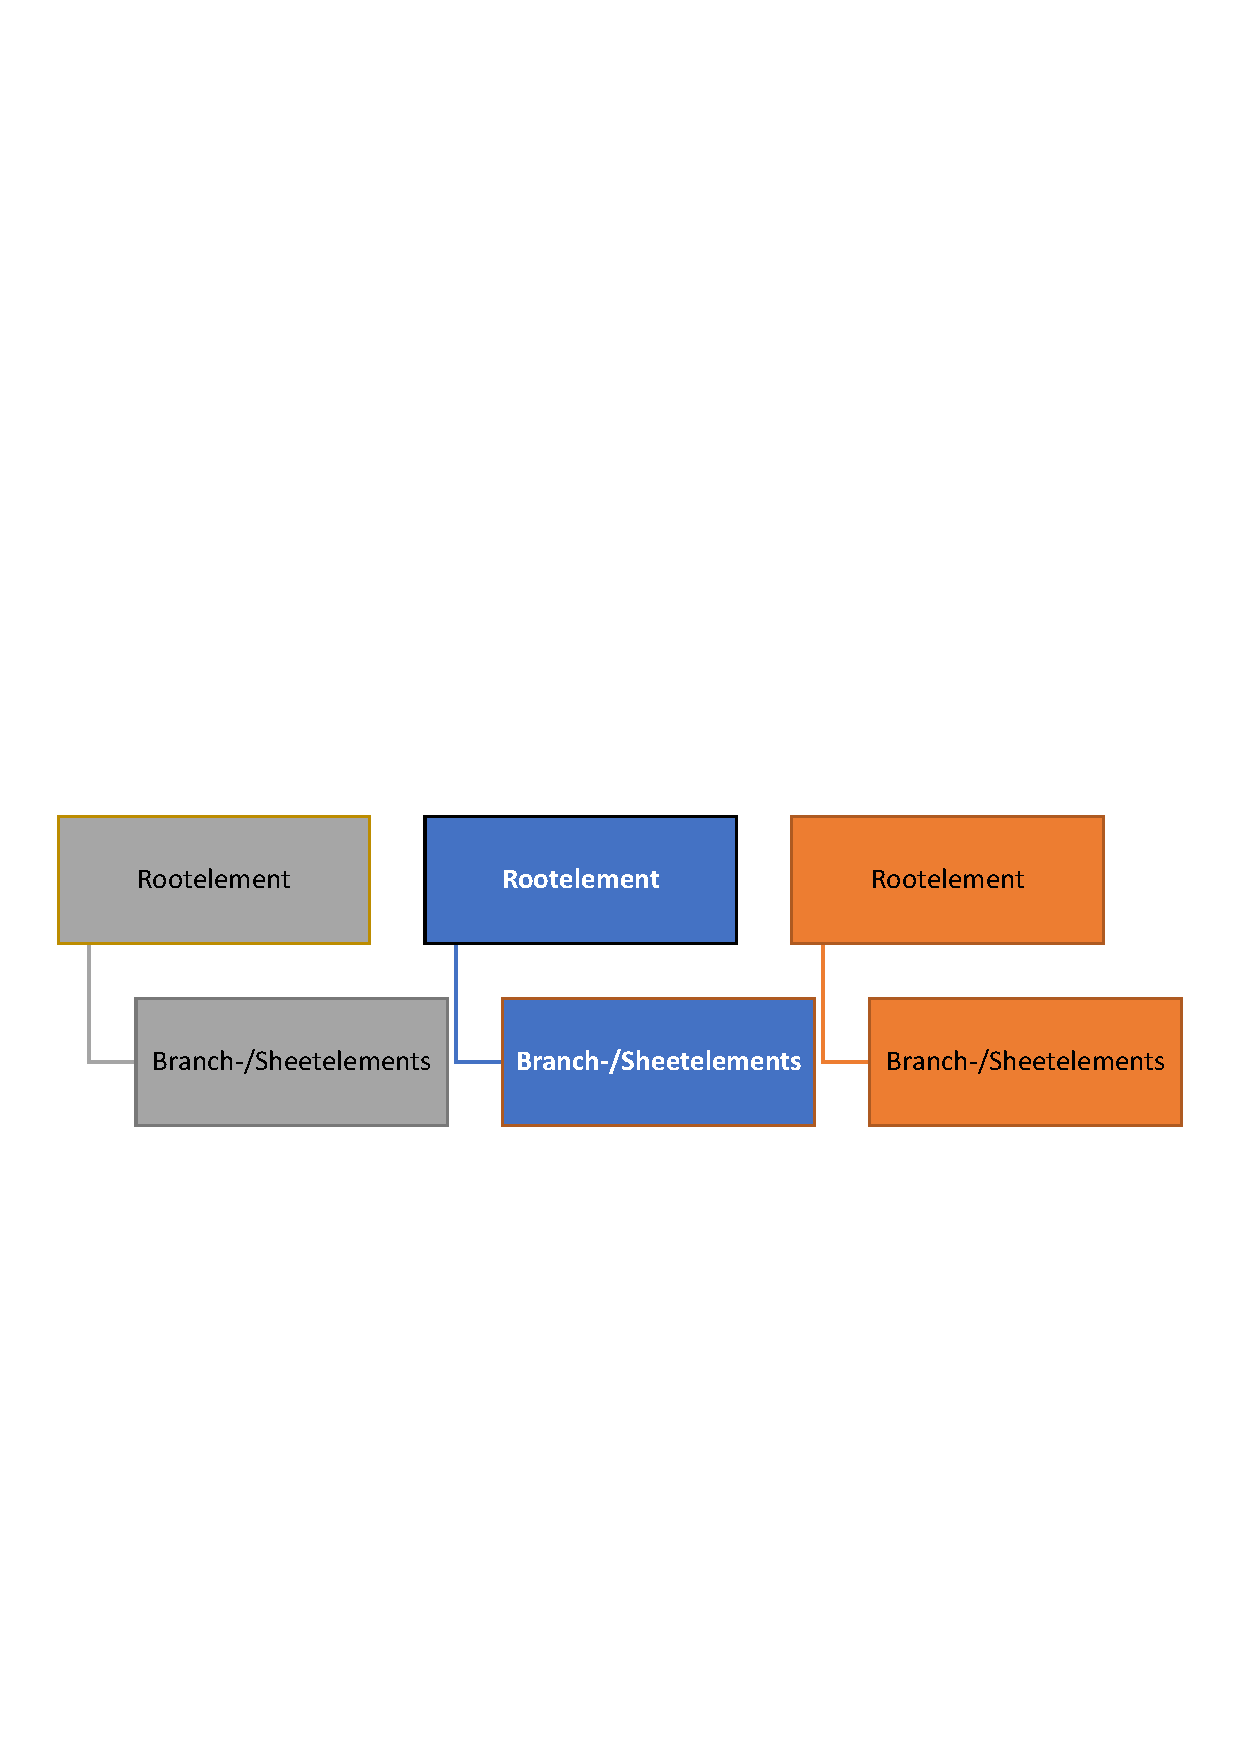
\includegraphics[width=0.8\textwidth]{Bilder/DB/Root_Branchelements.pdf}
\vspace{0em}
 \caption[Root-/Branchelements, gemäß ISA-S95]{Root-/Branchelements, gemäß ISA-S95}\label{fig:root_branch}
\end{figure}

\paragraph*{Anmerkung:} Die Grafiken dieses Abschnitts und denen im Anhang erheben keinen Anspruch auf \newline Vollständigkeit und Konsistenz. Die Erstellung der Grafiken wurden manuell in PowerPoint und keinem professionellem Tool erstellt, Tabellen und  Bezeichnungen haben demnach keine Referenzfunktion. Zur Darlegung der konzeptionellen Idee sollte die Güte der Qualität hinreichend sein.

Für die Verfahrenstechnik wurde im Rahmen dieses Projekts eine hierarchische Gliederung durchgeführt (siehe Abbildung \ref{fig:hierarchisch_vt}). Es wurden drei \textit{rootelements} definiert. Die unterschiedlichen Farben dienen im Verlauf dieses Abschnitts der visuellen Differenzierung der \textit{Rubriken}. 



\begin{figure}[h!] %[htbp!] 
\centering
%\vspace{-4em}
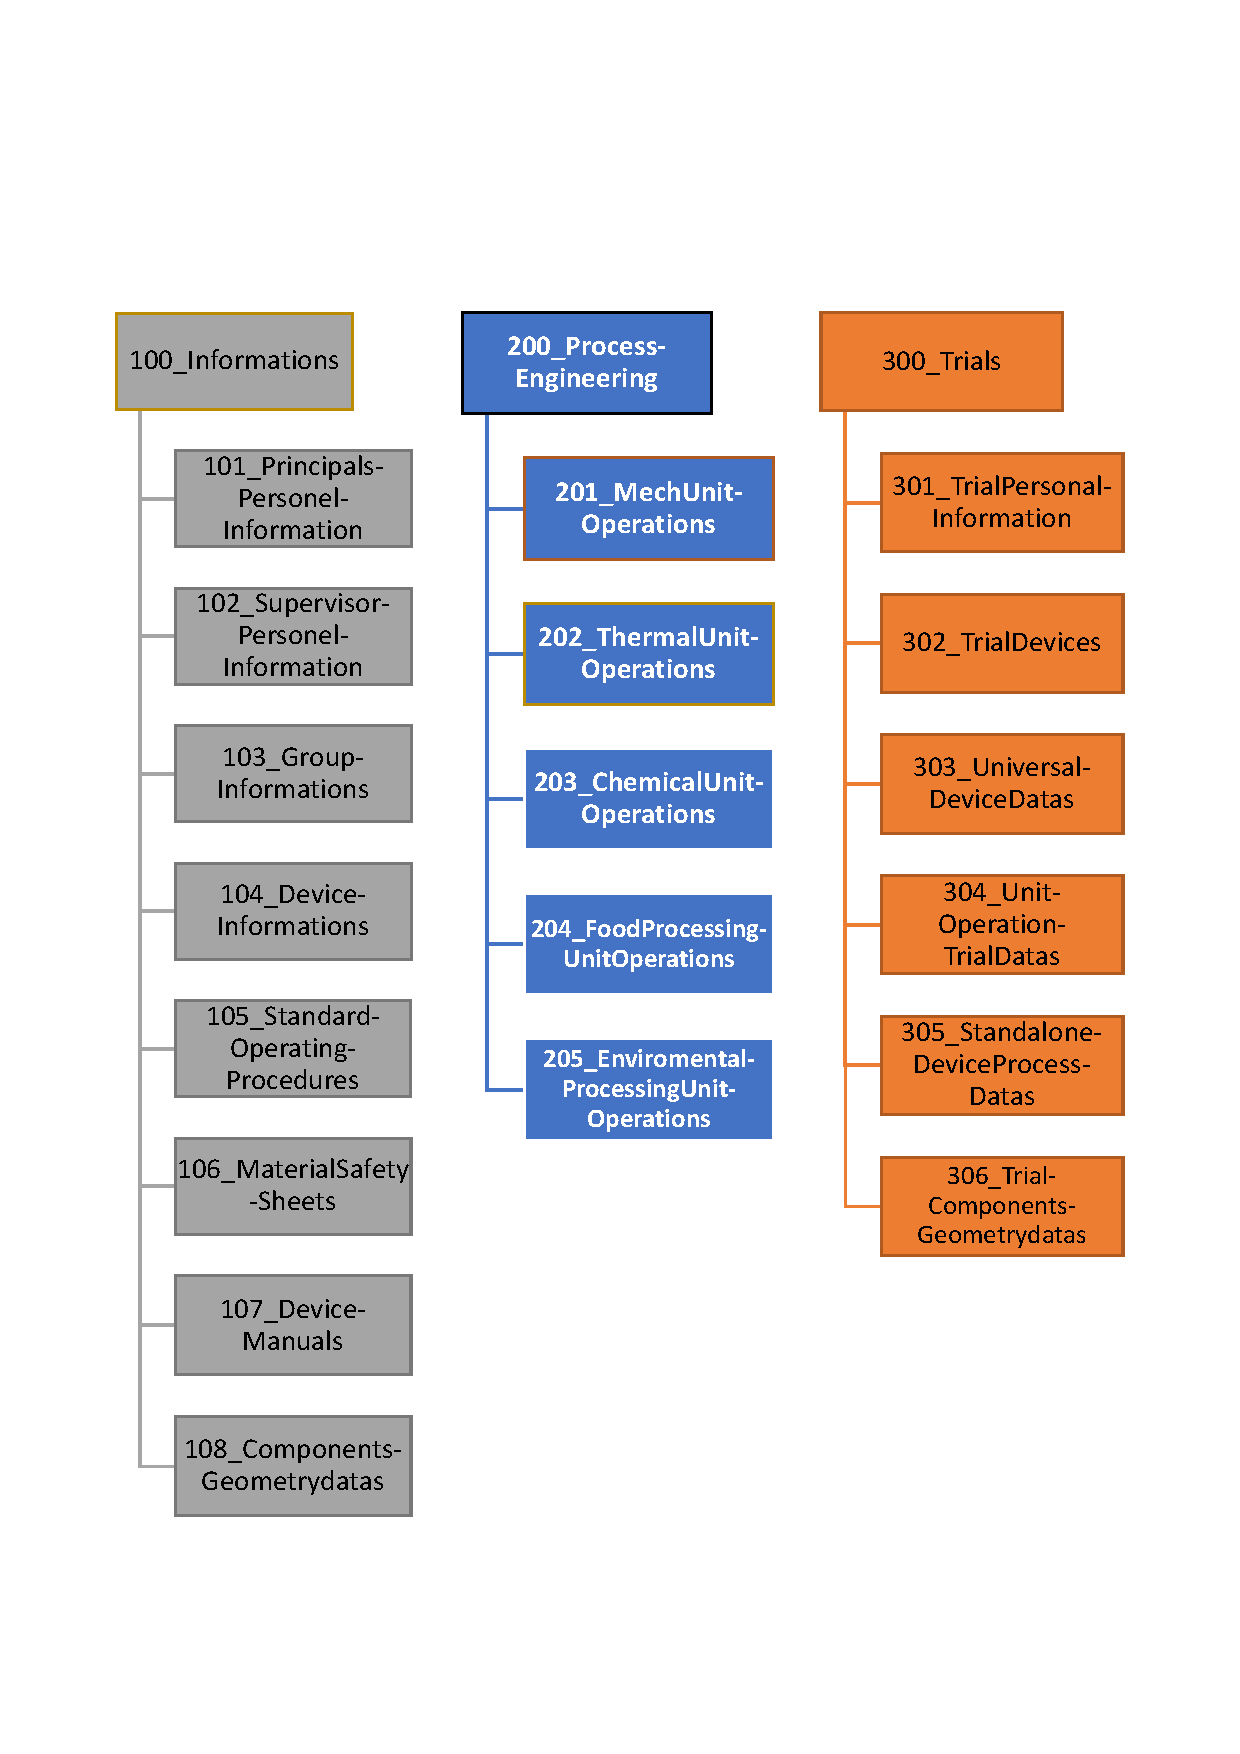
\includegraphics[width=.8\textwidth]{Bilder/DB/Labordatenstrukturdarstellung_im_ISA-95 Standard.pdf}
%\vspace{-4em}
 \caption[Labordatenstrukturdarstellung, angelehnt an ISA-S95]
 {Labordatenstrukturdarstellung, angelehnt an ISA-S95}\label{fig:hierarchisch_vt}
\end{figure}

\begin{itemize}
\item \textcolor{black!50}{{\Hypatia 100\_Informations}}
\item \textcolor{blue!90}{{\Hypatia 200\_ProcessEngineering}}
\item \textcolor{orange}{{\Hypatia 300\_Trials}}
\end{itemize}

Dem \textit{rootelement} {\Hypatia 100\_Informations} sind alle \textit{branch-} und \textit{sheetelements} untergeordnet, die allgemeine Informationen enthalten. Analog ist das für die definierten \textit{rootelemente} {\Hypatia 200\_ProcessEngineering} und {\Hypatia 300\_Trials} geschehen. In den sheetelements, die dem rootelement {\Hypatia 300\_Trials} untergeordnet sind, sind alle diskreten und kontinuierlichen Versuchsdaten und Parameter; wie bspw. Schüttgütspezifikationen, Druck und Volumenstrom sowie deren Kommentare am jeweiligen Zeitstempel, Geräte ID,  etc.; hinterlegt.
Allgemeine Informationen sind der Abbildung \ref{fig:hierarchisch_vt} zu entnehmen. Von dieser Grafik ist eine tabellarische Auflistung im Anhang vorhanden (siehe Tabelle \ref{tab:Labordatenstrukturdarstellung}).\\

An dieser Stelle wird exemplarisch die visualisierte \textit{Rubrik} {\Hypatia 100\_Informations} erläutert (siehe Abbildung~\ref{fig:100informations}). {\Hypatia 100\_Informations} \textbf{könnte} in allgemeine Informationen (\textit{engl. general informations}) und Laborinformationen (\textit{engl. laboratory informations}) unterteilt werden.  Zu den \textit{GeneralInformations} gehören unter anderem personelle Informationen ({\Hypatia 101 - 103}). Weitere Unterrubriken wurden nicht weiter aufgelistet. \textit{LaboratoryInformations} sind Informationen wie Versuchsanweisungen ({\Hypatia 105}), Sicherheitsdatenblätter ({\Hypatia 106}) etc. untergeordnet.\\



\begin{figure}[h!] %[htbp!] 
\centering
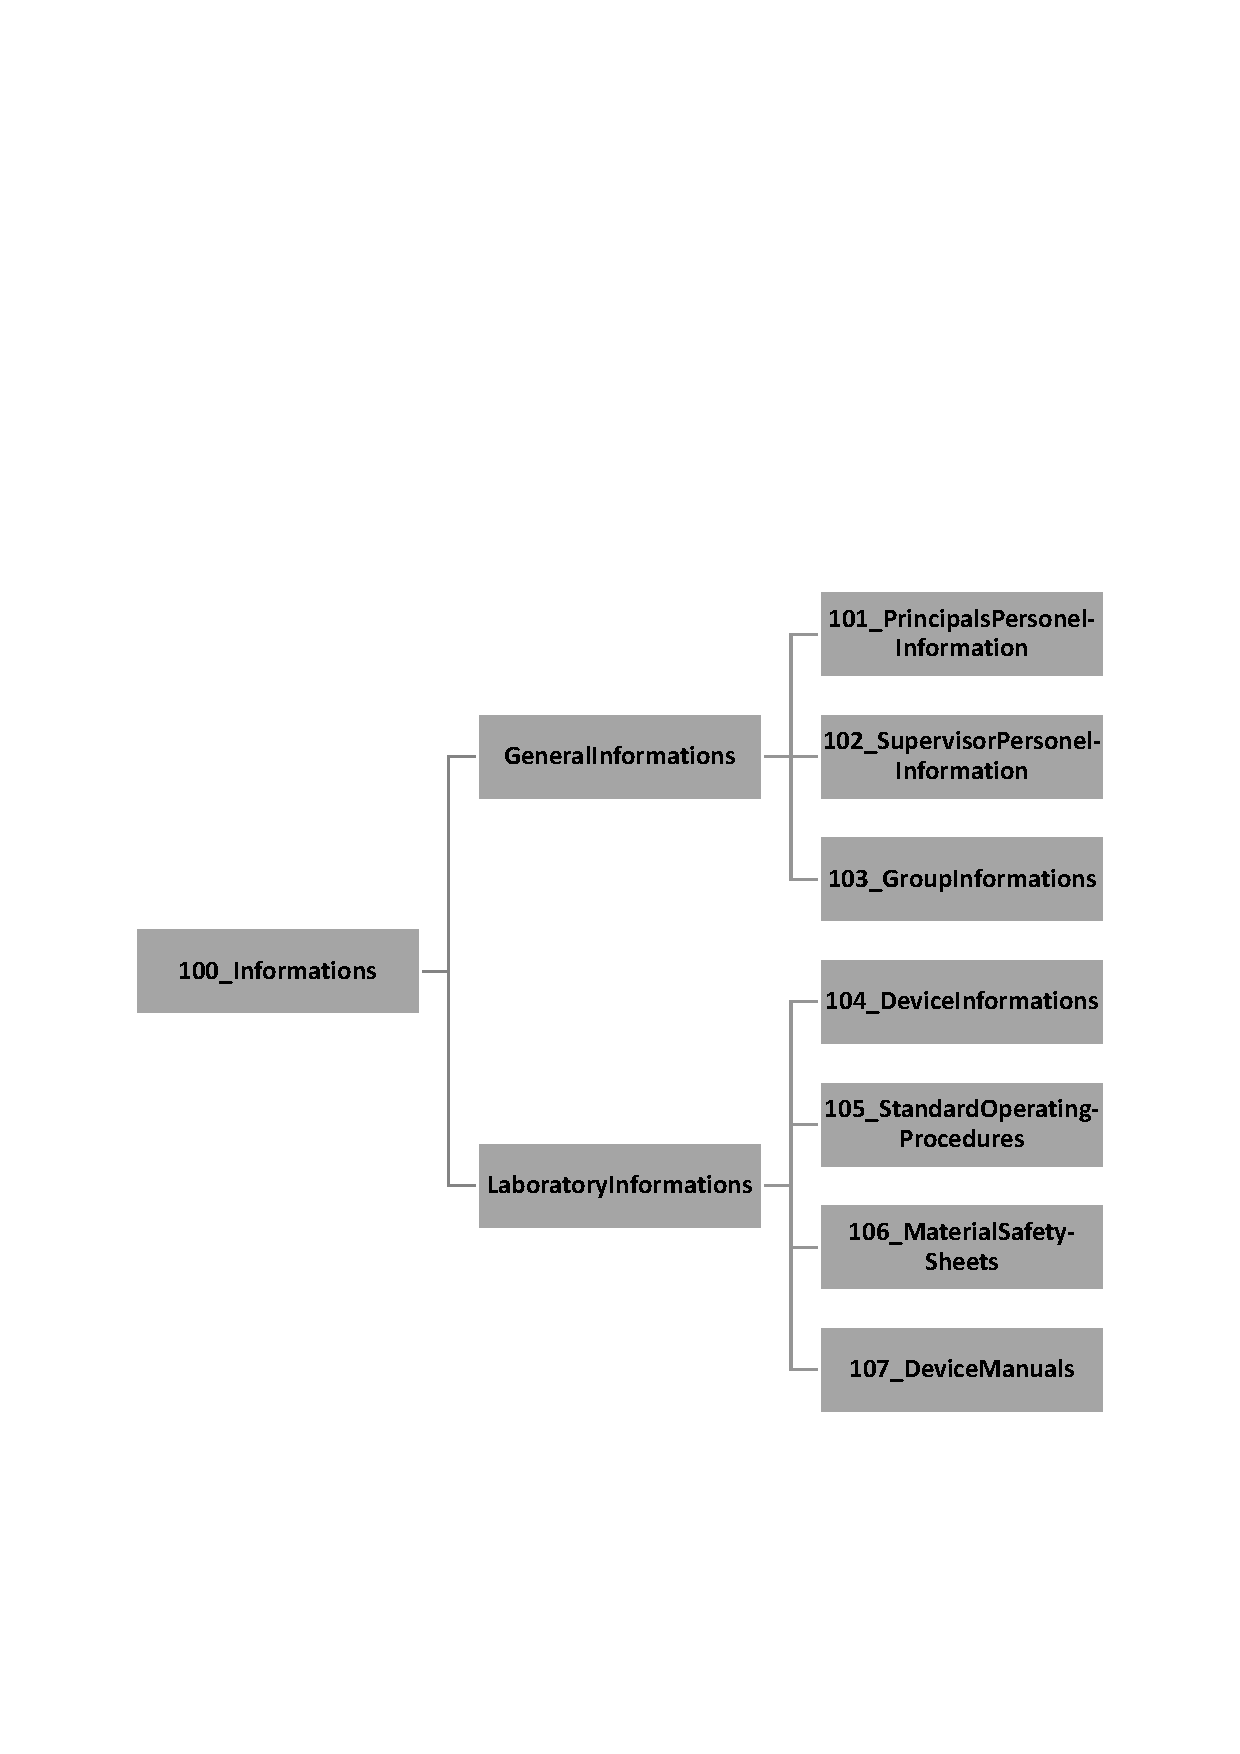
\includegraphics[width=0.9\textwidth]{Bilder/DB/ISA-S95_100_Informations.pdf}
\vspace{0em}
 \caption[100\_Informations, angelehnt an ISA-S95 und B2MML]
 {100\_Informations, angelehnt an ISA-S95}\label{fig:100informations}
\end{figure}

Den Abbildungen \ref{fig:200process} und \ref{fig:300trials} im Anhang kann die hierarchische Struktur der Rubriken 200\_ProcessEngineering und 300\_Trials entnommen werden.\\

Das \textit{Wold Batch Forum} hat eine Datenstruktur, mit dem Bezeichnung \textbf{B}usiness \textbf{To} \textbf{M}anufacturing \textbf{M}arkup \textbf{L}anguage (B2MML) entwickelt, auf der Basis von XML. XML-Dateien sind hierarchisch aufgegliedert. Jede XML- bzw. XSD-Datei (Dokument) besteht aus einem Wurzelelement (\textit{engl. rootelement}).  An dieser Stelle ist anzumerken, dass XML-Datenbanken dokumentbasiert funktionieren und hierarchische Strukturen aufweisen \cite{Verstehen2020}. Ein B2MML und BatchML Dokument (auf der Basis von XML) einer \textit{Rubrik} enthält demnach alle Informationen für eine bestimmte \textit{Rubrik}. B2MML bildet Geschäftsprozesse ab. Mit den B2MML und BatchML Vorlagen sind Unternehmen in der Lage ein individuelles Manufacturing Excecution System (MES) zu erstellen.\\

\begin{figure}[h!] %[htbp!] 
\centering
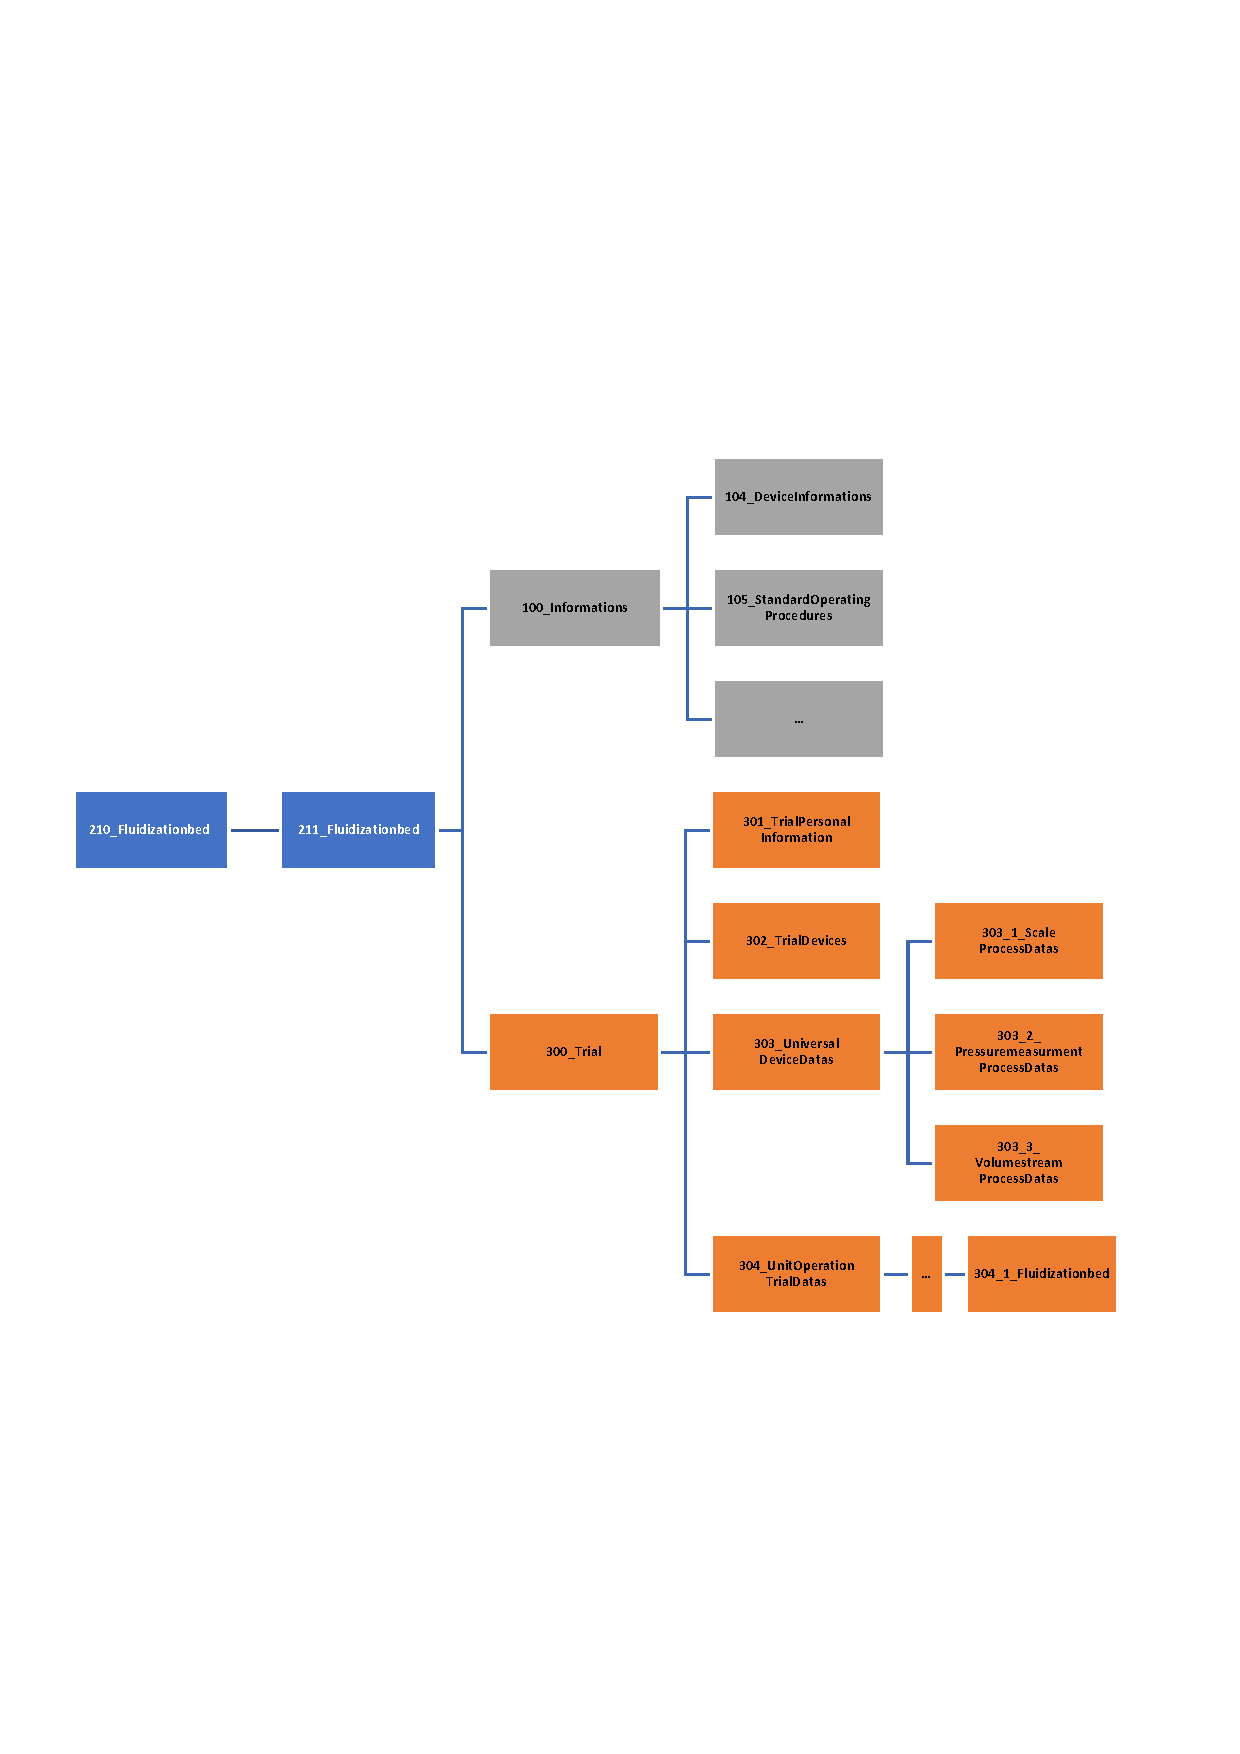
\includegraphics[width=1.05\textwidth]{Bilder/DB/wirbelschicht_hierarchisch_2.pdf}
\vspace{0em}
 \caption[Potentielle hierarchische Datenstruktur der Wirbelschicht (\textit{engl. fluidizationbed}) Unit Operation, angelehnt an ISA-S95 und B2MML]
 {Potentielle hierarchische Datenstruktur der Wirbelschicht (\textit{engl. fluidizationbed}) Unit Operation, angelehnt an ISA-S95 und B2MML}\label{fig:wirbelschicht hierarchisch}
\end{figure}

Wird das hierarchische Konzept auf das verfahrenstechnische Labor transferiert, dann könnte eine \textit{Rubrik} die Unit Operation Wirbelschicht (\textit{engl. fluidization bed}) sein. Die Struktur eines B2MML-Dokuments, zur Beschreibung eines \textbf{Wirbelschichtversuchsdurchlaufs}, könnte eine ähnliche Datenstruktur wie in Abbildung \ref{fig:wirbelschicht hierarchisch} dargestellt aufweisen. Daraus folgt, dass jeder Versuchstag bzw. Versuchsdurchlauf ein eigenes B2MML- bzw. XML-Dokument erhält. Gemäß Abbildung \ref{fig:wirbelschicht hierarchisch} würde die Unit Operation Wirbelschicht ({\Hypatia 210}) weitere \textit{branchelements} aufweisen, wie bspw. Wirbelschichttrocknen, Wirbelschichtagglomeration etc.. Das Labor der mechanischen Verfahrenstechnik der {\Hypatia HAW Life Sciences} hat nur eine Variation der Wirbelschicht, daher ist die erste und einzige Abzweigung ({\Hypatia 210}). An dieser Stelle kommen nun alle Elemente der obersten Hierarchiestufe ({\Hypatia 100, 300}). \textit{Branchelemente} der \textit{Rubrik} ({\Hypatia 100}) sollten jedoch nur Dokumentreferenzen sein, denn eine Redundanz dieser Daten hätte keinen Nutzen, sondern nur Aufwand zur Folge. Die nächste Hierarchieebene differenziert sich weiter auf und wird spezifischer. Auf der untersten eben wird es explizit. Im Rahmen dieses Beispiels würde die unterste Hierarchieebene die folgenden Elemente labeln:

\begin{enumerate}[resume, itemsep = -.1em, leftmargin=3.5em]	
\item[{\Hypatia 301}] Personenbezogenedaten des Versuchstags
\item[{\Hypatia 302}] Daten der notwendigen Geräte 
\item[{\Hypatia 303}] Erfasst alle zu erfassenen Daten. Darunter gehören diskrete sowie kontinuierliche \mbox{Daten}.
	\begin{enumerate}[ itemsep = -.1em]
	\item[{\Hypatia 303\_1}] Wiegedaten
	\item[{\Hypatia 303\_2}] Druckmessungsdaten
	\item[{\Hypatia 303\_3}] Volumenstommessungsdaten
	\end{enumerate}
	
\item[{\Hypatia 304}] Hier werden die prozessspezifischen Parameter dokumentiert
	\begin{enumerate}[ itemsep = -.1em]
	\item[{\Hypatia 304\_1}] In diesem Fall wären es die prozesspezifischen Parameter des Wirbelschichtversuchs an dem jeweiligen Versuchsstag
	\end{enumerate}
\end{enumerate}



Die Operation mit relationalen Datenbanken, auch SQL DB genannt, gestaltet sich in vielen Anwendungsfällen einfacher. Des Weiteren sind SQL DB am weitesten verbreitet und Programmschnittstellen sind in vielen Fällen für relationale Datenbanken (DB) ausgelegt. Transferiert man das hierarchische Konzept von ISA-S95 und B2MML auf eine SQL DB, dann bildet jedes einzelne Element eine eigenständige Tabelle ab. Eine dokumentenbasierte Datenbank würde beispielsweise eine ganze Unit Operation in einem Dokument zusammenfassen (vgl. Abbildung \ref{fig:wirbelschicht hierarchisch}). In einer SQL DB beschreiben demnach viele Tabellen eine Unit Operations bzw. einen Versuchsdurchlauf. Folglich ist der Aufwand der Tabellenerstellung möglicherweise höher, jedoch ist die Erstellung der abfragen via SQL einfach zu realisieren. Daher wird das ISA-S95, B2MML Konzept auf eine relationale Struktur transferiert (vgl. \ref{fig:sql_strukturentwurf}). Die Bezeichnungen in diesem Konzeptabschnitt wurden ins englische überführt.\\
 
In der Abbildung \ref{fig:sql_strukturentwurf} ist eine potentielle Datenstruktur für eine SQL Datenbank abgebildet. Es ist zu erkennen, dass Tabellen der unterschiedlichsten Rubriken; {\Hypatia 100\_Informations, 200\_ProcessEngineering, 300\_Trials}; in einer 1:N Beziehung zu einander stehen. Diese Struktur könnte den Wirbelschichtversuch hinreichend abbilden, denn:

\begin{enumerate}[ itemsep = -.1em, leftmargin=3.5em]
\item[{\Hypatia 100\_}] Informations stehen in relation mit der Unit Operation {\Hypatia 211\_Fluidizationbed}

	\begin{enumerate}[label = $\diamond$, itemsep = -.1em]
	\item Personelle Informationen werden erfasst.
	
		\begin{enumerate}[ itemsep = -.1em, leftmargin=2.5em]
		\item[{\Hypatia 101}] Auftraggeber (Professoren und Dozenten)
		\item[{\Hypatia 102}] Wissenschaftliche Mitarbeiter 
		\item[{\Hypatia 103}] Gruppeninformationen \\
		\end{enumerate}
		
	\item Allgemeine Informationen werden erfasst. Dateipfadreferenzen können hinterlegt werden. An dieser Stelle könnte eine dokumentenbasierte Datenbank Ihre Anwendung finden und die Archivierungsaufgabe besser lösen als eine SQL DB
	
		\begin{enumerate}[ itemsep = -.1em, leftmargin=2.5em]
		\item[{\Hypatia 104}] Geräteinformationen könnten sich auch Dokumentenbasiert abbilden lassen
		\item[{\Hypatia 105}] Versuchsanweisung (Standard Operating Procedures) 
		\item[{\Hypatia 106}] Materialdatenblätter
		\item[{\Hypatia 107}] Betriebsanweisungen von Geräten und Anlagen
		\item[{\Hypatia 108}] Geometrische Daten von Versuchsanlagen und Komponenten könnten Dokumentenbasiert möglicherweise effizienter archiviert werden. Eine Möglichkeit via SQL ist es für jedes Komponent eine Tabelle zu generieren. Dokumentenbasiert würde ein Bauteil ein Dokument erhalten und alle Komponenten enthalten.
		
	\end{enumerate}
	\end{enumerate}
\end{enumerate}
\pagebreak



\begin{enumerate}[resume, itemsep = -.1em, leftmargin=3.5em]	
\item[{\Hypatia 300\_}] Trials werden via diverser Tabellen erfasst
	\begin{enumerate}[ itemsep = -.1em]
	\item[{\Hypatia 300}] könnte organisatorische Daten die versuchstagbezogen sind, wie bspw. das Datum oder der wievielte Versuch (sollte eine Gruppe mal gescheitert sein), aber auch das Hochladedatum sowie eine Speicherortreferenz erfassen. Für die Speicherung der Protokolle könnte ebenfalls ein dokumentenbasierte DB Lösung zum Einsatz kommen.
	\item[{\Hypatia 301}] Personenbezogene Informationen pro Versuchstag werden erfasst
	\item[{\Hypatia 302}] könnte bei redundanten Apparaten, Geräten, Aggregaten relevant sein
	\item[{\Hypatia 303}] Erfasst alle zu erfassenen Daten. Darunter gehören diskrete so wie kontinuierliche \mbox{Daten}.
	
	\begin{enumerate}[ itemsep = -.1em]
	\item[{\Hypatia 303\_1}] Wiegedaten
	\item[{\Hypatia 303\_2}] Druckmessungsdaten
	\item[{\Hypatia 303\_3}] Volumenstommessungsdaten
	
		\begin{enumerate}[label=--, itemsep = -.5em]
		\item An der Stelle können diveser Kommentarfelder eingefügt werden, die einen Versuch beschreiben wie Subjektive Beobachtungen, die Wirbelschichthöhte und die Wirbelschichtporösität.
		\end{enumerate}
	\item[{\Hypatia 304\_1}] Hier werden die prozessspezifischen Parameter dokumentiert
	\end{enumerate}
		\end{enumerate}
\end{enumerate}

Im Anhang befindet sich eine Grafik, die verschiedene Abstraktionsebenen vermischt darstellt (siehe Abbildung \ref{fig:mixed_abstraction}). Auf der untersten Abstraktionsebene wären die expliziten Tabellen aufzufinden. Eine beispielhafte Zusammenstellung ist dem Anhang, der Abbildung \ref{fig:sql_explizit} zu entnehmen.


\begin{figure}[p!] %[htbp!] 
\centering
\vspace{-2em}
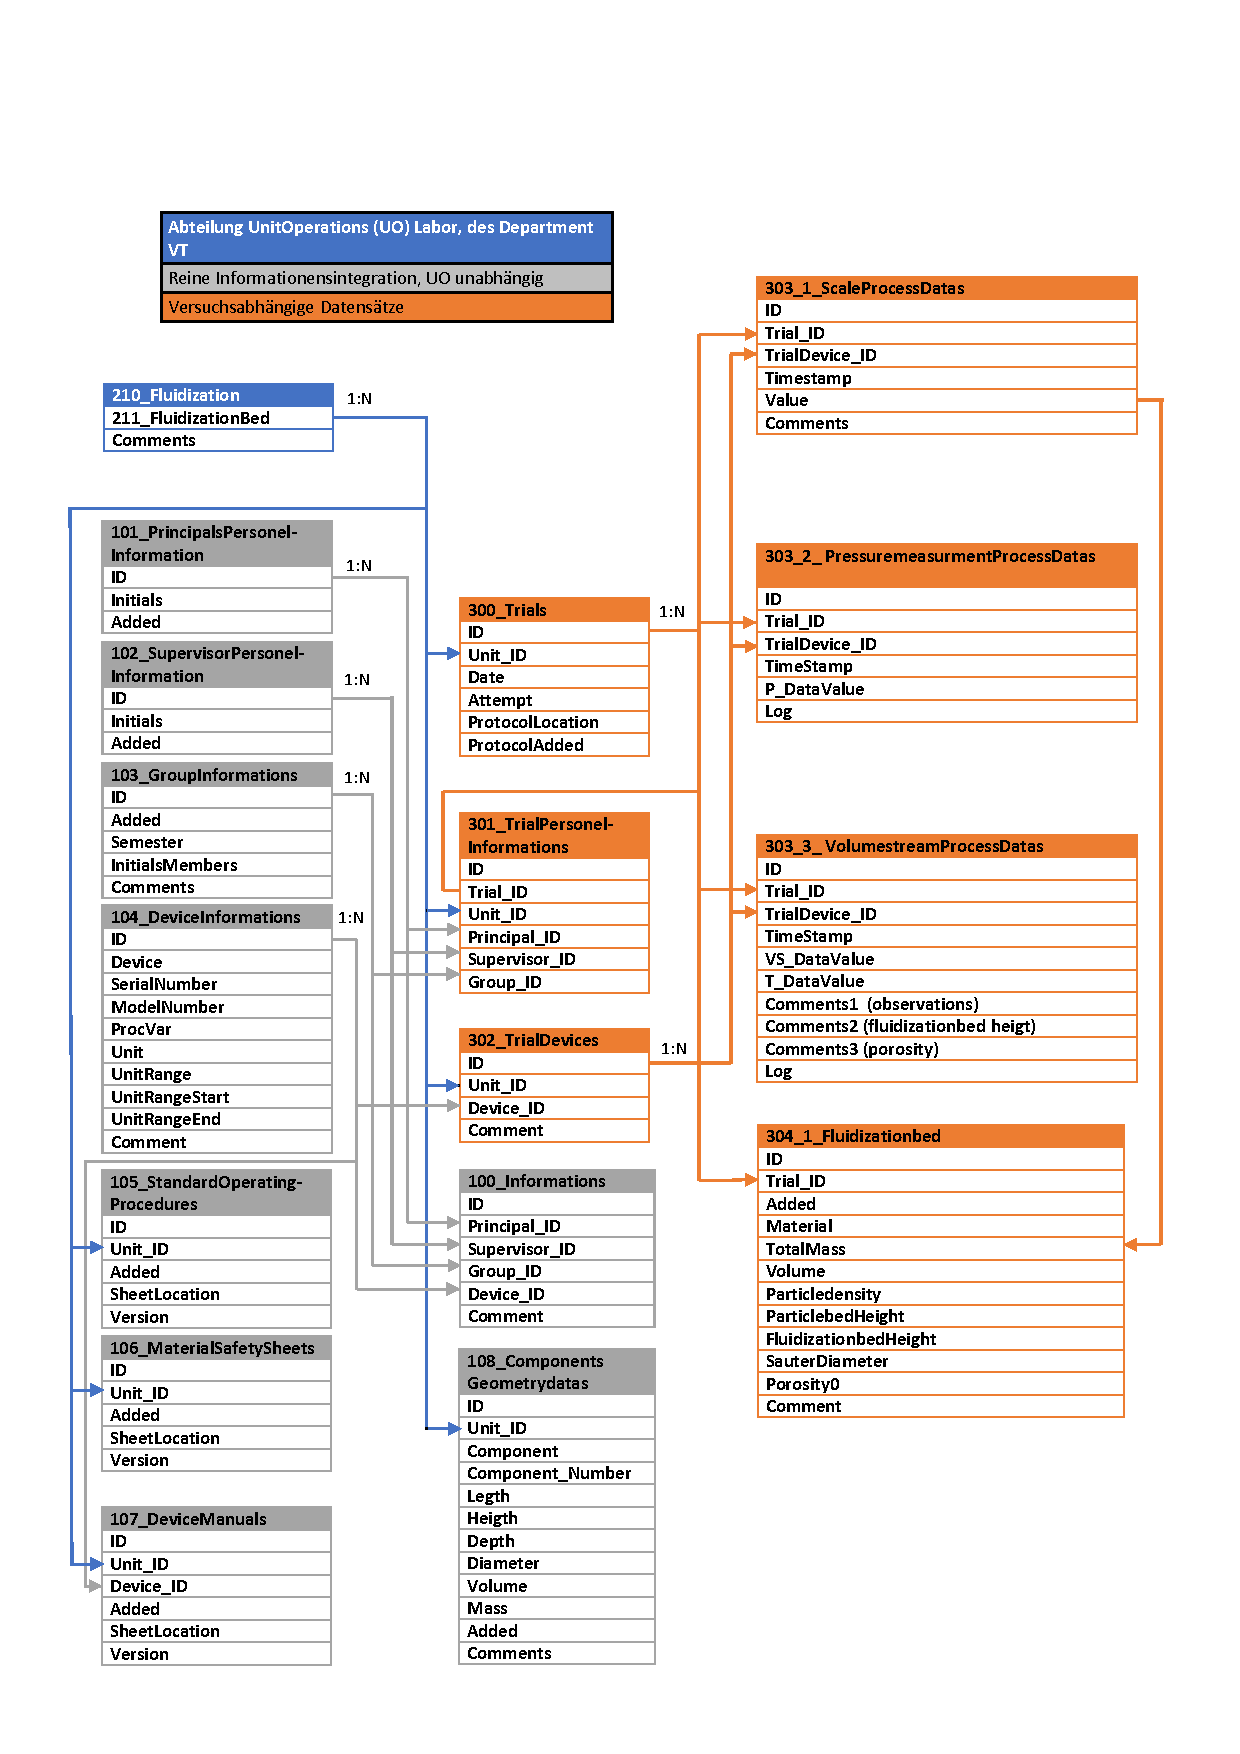
\includegraphics[width=1.02\textwidth]{Bilder/DB/wirbelschicht_sql.pdf}
\vspace{-2em}
 \caption[Datenstrukturentwurf einer relationalen Datenbank zur Beschreibung der Wirbelschicht Unit Operation, angelehnt an ISA-S95 und B2MML]
 {Datenstrukturentwurf einer relationalen Datenbank zur Beschreibung der Wirbelschicht Unit Operation, angelehnt an ISA-S95 und B2MML}\label{fig:sql_strukturentwurf}
\end{figure}

\subsubsection{Fazit}

Im Rahmen der Anwendungsfälle im Hochschulalltag könnten SQL Datenbanken den Anforderungen genügen. Das Know-How mit dieser standardisierten Datenbank Technologie ist auf andere Softwaretechnologien transferierbar. Es sollte auch möglich sein, die Erstellung einer Datenbank, im Rahmen studentischer Arbeiten, zu delegieren. Des Weiteren ist auch im Verlauf des \textit{Digitalisierungsprozess} eine Hybridlösung denkbar. 